\subsection{Kiến trúc hệ thống}
\subsubsection{Phân tích kiến trúc hệ thống phổ biến hiện nay}
Hiện nay, có nhiều kiến trúc phần mềm khác nhau, mỗi loại có ưu và nhược điểm riêng, phù hợp với các loại dự án và yêu cầu cụ thể. Dưới đây là một số kiến trúc phần mềm phổ biến và các điểm chính của chúng:
\begin{enumerate}
    \item Kiến trúc Monolithic
    \begin{itemize}
        \item \textbf{\textit{Định nghĩa:}} Kiến trúc monolithic là một mô hình truyền thống trong đó toàn bộ ứng dụng được xây dựng như một đơn vị duy nhất, tích hợp chặt chẽ.
        \item \textbf{\textit{Điểm chính:}} 
        \begin{itemize}
            \item Đơn giản để phát triển, triển khai và kiểm thử
            \item Hiệu suất tốt do không có overhead của network calls
            \item Khó mở rộng và bảo trì khi ứng dụng phức tạp
            \item Khó áp dụng công nghệ mới cho từng phần của ứng dụng
        \end{itemize}
        \item \textbf{\textit{Ví dụ:}} Một ứng dụng web PHP truyền thống, nơi tất cả chức năng (UI, business logic, data access) đều nằm trong cùng một codebase.
    \end{itemize}
    \item Kiến trúc Microservices
    \begin{itemize}
        \item \textbf{\textit{Định nghĩa:}} Kiến trúc microservices chia nhỏ ứng dụng thành các dịch vụ độc lập, mỗi dịch vụ chịu trách nhiệm cho một chức năng cụ thể và có thể được phát triển, triển khai độc lập.
        \item \textbf{\textit{Điểm chính:}} 
        \begin{itemize}
            \item Dễ dàng mở rộng và bảo trì từng service riêng biệt
            \item Cho phép sử dụng công nghệ phù hợp nhất cho mỗi service
            \item Tăng cường khả năng chịu lỗi của hệ thống
            \item Phức tạp hơn trong việc quản lý và điều phối các service
        \end{itemize}
        \item \textbf{\textit{Ví dụ:}} Netflix sử dụng kiến trúc microservices, với các service riêng biệt cho việc xử lý video, quản lý người dùng, đề xuất nội dung, v.v.
    \end{itemize}
    \item Kiến trúc Client-Server (Multitier)
    \begin{itemize}
        \item \textbf{\textit{Định nghĩa:}} Kiến trúc client-server chia ứng dụng thành các tầng (tiers) riêng biệt, thường bao gồm tầng trình bày (presentation), tầng logic nghiệp vụ (business logic), và tầng dữ liệu (data).
        \item \textbf{\textit{Điểm chính:}} 
        \begin{itemize}
            \item Phân tách rõ ràng giữa các tầng chức năng
            \item Dễ dàng mở rộng từng tầng độc lập
            \item Cải thiện bảo mật bằng cách kiểm soát quyền truy cập giữa các tầng
            \item Có thể trở nên phức tạp khi số lượng tầng tăng lên
        \end{itemize}
        \item \textbf{\textit{Ví dụ:}} Một ứng dụng web ba tầng điển hình bao gồm frontend (React), backend API (Node.js), và cơ sở dữ liệu (PostgreSQL).
    \end{itemize}
    \item Kiến trúc Event-Driven
    \begin{itemize}
        \item \textbf{\textit{Định nghĩa:}} Kiến trúc event-driven là một mô hình trong đó việc tạo ra, phát hiện, tiêu thụ và phản ứng với các sự kiện là cốt lõi của hệ thống.
        \item \textbf{\textit{Điểm chính:}} 
        \begin{itemize}
            \item Tách rời các thành phần hệ thống, giảm sự phụ thuộc trực tiếp
            \item Khả năng mở rộng và linh hoạt cao
            \item Dễ dàng thêm chức năng mới mà không ảnh hưởng đến các thành phần hiện có
            \item Có thể phức tạp trong việc theo dõi luồng xử lý và debug
        \end{itemize}
        \item \textbf{\textit{Ví dụ:}} Hệ thống thương mại điện tử, khi một đơn hàng được đặt, một sự kiện "OrderPlaced" được phát ra, kích hoạt các quy trình xử lý khác như cập nhật kho, gửi email xác nhận, v.v.
    \end{itemize}
    \item Kiến trúc Serverless
    \begin{itemize}
        \item \textbf{\textit{Định nghĩa:}} Kiến trúc serverless cho phép phát triển và chạy ứng dụng mà không cần quản lý trực tiếp máy chủ, tập trung vào việc viết code cho các chức năng (functions) cụ thể.
        \item \textbf{\textit{Điểm chính:}} 
        \begin{itemize}
            \item Giảm chi phí vận hành và bảo trì hạ tầng
            \item Tự động mở rộng theo nhu cầu sử dụng
            \item Chỉ trả tiền cho tài nguyên thực sự sử dụng
            \item Có thể gặp vấn đề về cold start và vendor lock-in
        \end{itemize}
        \item \textbf{\textit{Ví dụ:}} Một ứng dụng xử lý ảnh sử dụng AWS Lambda để thực hiện các tác vụ như resize, filter, và lưu trữ ảnh khi người dùng tải lên.
    \end{itemize}
\end{enumerate}
\subsubsection{Lựa chọn kiến trúc hệ thống}
Dựa trên yêu cầu của hệ thống, nhóm sử dụng kiến trúc kết hợp giữa Microservices và Multitier Client-Server. Cụ thể như sau:
\begin{enumerate}
    \item Presentation Tier (Client Tier):
    \begin{itemize}
        \item Frontend: Vue.js application
        \item Giao diện người dùng cho sinh viên và giảng viên
        \item Tương tác với backend thông qua RESTful API
    \end{itemize}
    \item Application Tier:
    \begin{enumerate}
        \item API Gateway:
        \begin{itemize}
            \item Nginx hoặc API Gateway mã nguồn mở
            \item Xử lý authentication, authorization và định tuyến requests đến các microservices
        \end{itemize}

    \item Microservices (tất cả được xây dựng bằng Fast API):
    \begin{itemize}
        \item User Service:
        \begin{itemize}
            \item Quản lý thông tin người dùng
            \item Xác thực và phân quyền
        \end{itemize}
        \item Course Management Service:
        \begin{itemize}
            \item CRUD operations cho khóa học, module, bài học
            \item Quản lý nội dung học tập
        \end{itemize}
        \item Recommentation Learning Service:
        \begin{itemize}
            \item Đề xuất learning items dựa trên dữ liệu người dùng
        \end{itemize}
        \item AI Tutor Service:
        \begin{itemize}
            \item Tích hợp Langchain để xây dựng gia sư AI
            \item Xử lý các yêu cầu liên quan đến hỗ trợ lập trình và giải thích mã nguồn
        \end{itemize}
        \item Exercise Generation Service:
        \begin{itemize}
            \item Sử dụng Langchain để tạo bài tập và test cases tự động
            \item Đánh giá bài làm của người học
        \end{itemize}
        \item Progress Tracking Service:
        \begin{itemize}
            \item Theo dõi và ghi nhận tiến độ học tập
            \item Tạo báo cáo học tập
        \end{itemize}
    \end{itemize} 
    \end{enumerate}
    \item Data Tier:
    \begin{enumerate}
        \item Persistence Layer:
        \begin{itemize}
            \item PostgreSQL: Lưu trữ dữ liệu có cấu trúc (thông tin người dùng, khóa học, bài học)
            \item Neo4j: Lưu trữ và quản lý mối quan hệ giữa các learning items, hỗ trợ tạo lộ trình học tập
            \item AWS S3: Lưu trữ tài liệu học tập, video bài giảng
        \end{itemize}
        \item Caching Layer: 
        \begin{itemize}
            \item Redis: Cải thiện hiệu suất và giảm tải cho database
        \end{itemize}
    \end{enumerate}
\end{enumerate}
\textbf{\textit{Phân tích nguyên nhân:}}
\par \begin{itemize}
    \item Phân chia trách nhiệm rõ ràng: Mỗi dịch vụ có một nhiệm vụ cụ thể, dễ bảo trì và phát triển. Ví dụ, FastAPI quản lý API, Langchain xử lý AI, PostgreSQL và Neo4j quản lý dữ liệu.
    \item Dễ mở rộng: Mỗi dịch vụ có thể mở rộng riêng lẻ khi tải tăng lên, như tăng số lượng instances của FastAPI khi số người dùng tăng.
    \item Triển khai linh hoạt: Thay đổi hoặc thêm công nghệ mới dễ dàng mà không ảnh hưởng đến toàn hệ thống.
\end{itemize}
\textbf{\textit{Không dùng:}}
\begin{itemize}
    \item Monolithic vì khó mở rộng, bảo trì, và tích hợp công nghệ mới.
    \item Event-driven vì phức tạp khi quản lý trạng thái trực tiếp và đồng bộ.
    \item Serverless do phụ thuộc nhà cung cấp, chi phí cao khi tải tăng, và hạn chế tùy chỉnh hiệu suất.
\end{itemize}
Như vậy, ta có luồng hoạt động của hệ thống như sau:
\begin{itemize}
    \item Người dùng tương tác với frontend Vue.js (Presentation Tier).
    \item Requests được gửi đến API Gateway trong Application Tier.
    \item API Gateway xác thực và định tuyến requests đến microservice phù hợp.
    \item Microservices trong Application Tier xử lý business logic:
    \begin{itemize}
        \item Gọi đến Persistence Layer trong Data Tier để lưu trữ hoặc truy xuất dữ liệu.
        \item Sử dụng Caching Layer để tối ưu hiệu suất truy vấn.
    \end{itemize}
    \item Kết quả được trả về cho frontend thông qua API Gateway.
\end{itemize}
\textbf{\textit{Tóm lại,}} kiến trúc kết hợp ưu điểm của Microservices và Multitier tận dụng tối đa các công nghệ đã được chọn để xây dựng một hệ thống học tập trực tuyến thông minh, có khả năng mở rộng cao và linh hoạt. Việc phân chia rõ ràng giữa các tiers và microservices giúp dễ dàng phát triển, bảo trì và mở rộng hệ thống trong tương lai.
\begin{figure}[H]
    \centering
    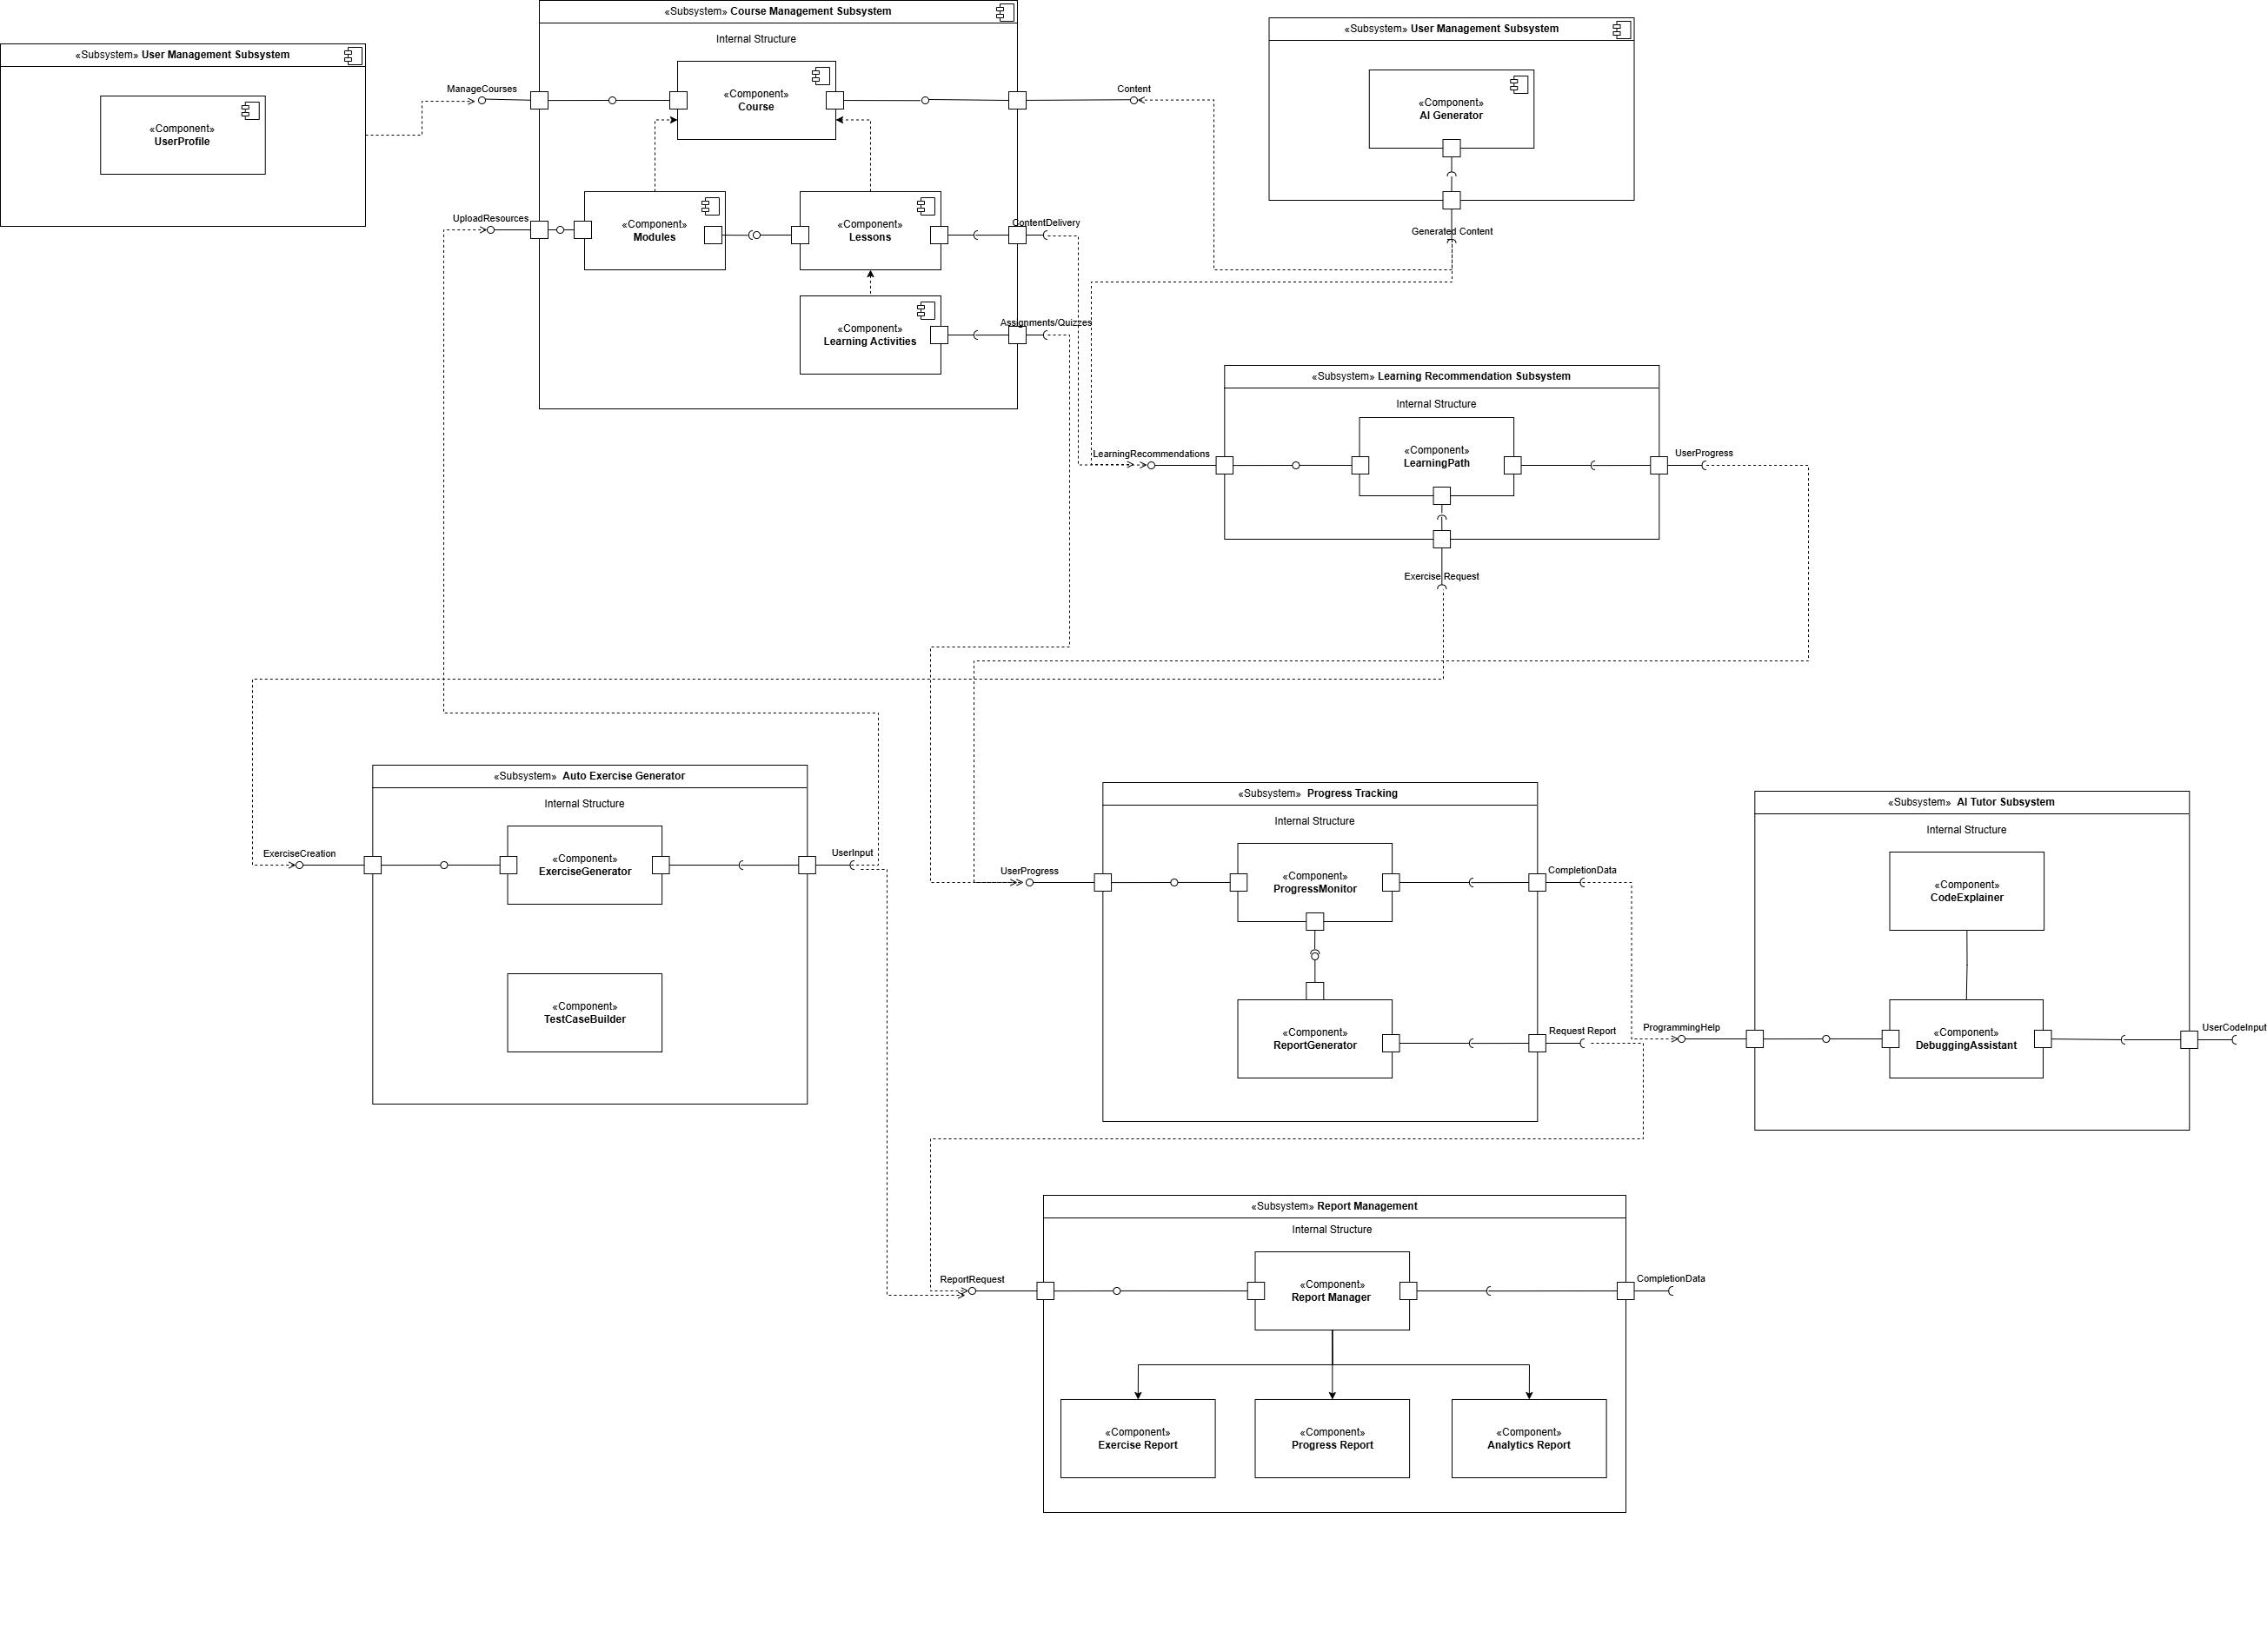
\includegraphics[width=\linewidth]{Images/component_diagram/component-All.drawio.png}
    \caption{Component-based Diagram cho toàn bộ hệ thống}
    \label{fig:enter-label}
\end{figure}
\begin{figure}[H]
    \centering
    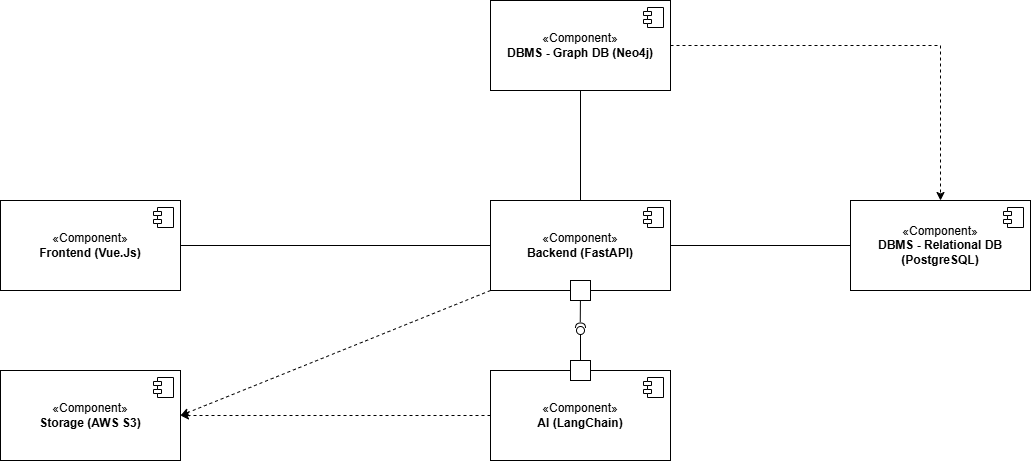
\includegraphics[width=\linewidth]{Images/component_diagram/component-Selected technologies.drawio.png}
    \caption{Component-based Diagram cho những công nghệ được chọn}
    \label{fig:enter-label}
\end{figure}